\documentclass[a4paper,12pt]{article}

\usepackage[margin=90pt]{geometry}
\usepackage[T1,T2A]{fontenc}
\usepackage[utf8]{inputenc}
\usepackage[maxbibnames=99]{biblatex}
\usepackage[bulgarian]{babel}
\usepackage[unicode]{hyperref}
\usepackage{enumitem}
\usepackage{upgreek}
\usepackage{url}
\usepackage{graphicx}
\usepackage{mathtools}
\usepackage{indentfirst}
\usepackage[autostyle=false]{csquotes}
\usepackage{textcomp, gensymb}
\usepackage{subcaption}
\usepackage{bm,amsmath,amsfonts,amssymb}

\addbibresource{./references.bib}
\graphicspath{ {./img/} }

\DeclareUnicodeCharacter{0301}{\'{e}}


\DeclareCaptionFormat{custom}
{%
    \textbf{\small #1#2}\textit{\small #3}
}
\captionsetup{format=custom}

\begin{document}
\title{
    Пред-дипломна работа\\
    \large Откриване на подобни и идентични изображения в архиви на музеи}
\author{Иван Христов, ФН - 2MI3400066}

\maketitle


\pagebreak

% =============================================================================================================
\section{Увод}

% *************************************************************************************************************
\subsection{Актуалност на проблема и мотивация}

С течение на времето се правят находки с културна стойност. Осезаема част от тях са под формата на снимки, съдържащи исторически лица редом с характерните за тяхната среда обекти. Анализът на такива снимки изисква участието на историци и етнографи. Следователно процесът е трудоемък и с възможност за допускане на субективни грешки. Дублициране на исторически изображения е възможно, било то поради невнимание при сканиране или сливане на архиви с общи снимки. Повтарянето на изображения е възможно да доведе до излишен човешки труд и съответно загубено време.

\bigbreak

Пример за институция с този пробем е Троянският музей. Той разполага с архив от \textit{4TB} снимки в \textit{JPG} формат, чиито източници варират. Някой от тях са заснети чрез фотоапарат, докато други са сканирани. Съответно те са подложени на различни афинни трансформации (ротация, скалиране, отместване и др.), дисторция и илюминация. Пример за това е, че размерите на изображенията варират от около \textit{200KB} до около \textit{10MB}. Троянският музей специализира в народните занаяти, но има и богата сбирка от градски изображения - някои от които са с тълпи от хора, други с малко на брой субекти. Съответно детайлността на изображенията варира, което би могло да бъде проблем при наличие на ниска резолюция на изображенията. Снимките от музея са исторически, съответно има наличие на черно-бели и цветни изображения.

\bigbreak

Архивът на Троянският музей със своето разнообразие е достатъчно представителен за проблема, но той далеч не е единственият такъв. Пример за подобно множество от снимки е това на Народната библиотека в Пловдив. Следователно дедупликацията на исторически изображения е проблем, чиято автоматизация би имала културен и исторически принос на много места.

% *************************************************************************************************************
\subsection{Цел и задачи на пред-дипломната работа}

На най-абстрактно ниво бизнес целта на пред-дипломната работа е да намали времето инвестирано от историци в анализ на изображения. Това не означава замяна на такива специалисти, а напротив - улеснение на тяхната работа. Постигането на тази цел е възможно, използвайки комбинация от похвати познати в обработката на изображения и изкуствения интелект. В такъв ред на мисли тази работа предоставя обзор на такива похвати, избор на комбинация от тях, обоснован от бизнес контекста, и изграждането на общодостъпен инструмент имплементиращ ги.

\bigbreak

Дедупликацията на исторически изображения е един начин да се помогне на историците. Съществува множество от други проблеми - като разпознаване на лица от снимки, категоризиране и откриване на обекти, коригиране на дефекти и прочие. Съответно тази работа може да се разглежда като стъпка към изграждането на един по-голям инструмент за разрешаването на разнообразни проблеми в работата на историците.

% *************************************************************************************************************
\subsection{Очаквани ползи от реализацията}


% *************************************************************************************************************
\subsection{Структура на преддипломната работа}

% =============================================================================================================
\section{Преглед на предметната област}

% *************************************************************************************************************
\subsection{Основни дефиниции}

В тази секция се обяснява какво е задачата за дедупликация на изображения, давайки дефиниция на проблемите пред нея.

\bigbreak

Казваме, че две изображения са \textbf{идентични} когато те са фотографични копия на едно оригинално изображение. Фотографично копие на оригинално изображение се получава чрез прилагане на трансформации върху него, сред които афинни, контрастни, илюминационни, дистортни и компресивни. Примери за практически методи за получаването на фотографични копия са презаснемане на изображение чрез камера или скенер. Терминът фотографично копие е \textbf{размит}, като той означава максимално сходство между изображение копие и неговия оригинал относно детайлност (виж \hyperref[def:imdetail]{деф.}), контраст и цветове.

\bigbreak

Трябва да се прави разлика между идентични и подобни изображения. Нека $A'$ и $B'$ са изображения, като съответно $A'$ е фотографично копие на $A$ и $B'$ е фотографично копие на $B$. Нека $A$ и $B$ не са производни на други изображения, т.е. са оригинални. Казваме, че изображение $A'$ е \textbf{подобно} на изображение $B'$, ако $A$ и $B$ се различават съвсем малко по детайлност (виж \hyperref[def:imdetail]{деф.}), контраст и цветове. Пример за практически метод за получаване на подобни изображения е няколкократно заснемане на изображение в рамките на секунда. Пример за разлика в детайлност е ако на снимка $A$ има човек с отворени очи, а на $B$ той е със затворени. Задачата за дедупликация се занимава с откриването на \textbf{идентични} изображения. На практика алгоритмите за откриване на дуплицирани изображения третират подобните и идентичните изображения по еднакъв начин. Това се налага поради размитостта на понятията. 

\bigbreak

\label{def:imdetail}Детайлността на едно изображение се представя чрез неговите точки на интерес. Точка на интерес наричаме регион от изображението, който е устойчив на математически операции, защото е богат на информация, има ясно дефинирано разположение в пространството и е стабилен на локални и глобални трансформации в изображението (виж \cite{sift}). Нека имаме изображение $A$ с две фотографични копия $B$ и $C$ и точка на интерес $\alpha$. Лесно може да се определи, къде в $B$ и къде в $C$ е проектирана $\alpha$. Следователно дефиницията за подобие/идентичност между две изображения може да се преформулира по следния начин - нека $A$ и $B$ са изображения; казваме, че $A$ и $B$ са подобни/идентични ако количеството споделени точки на интерес във всяко едно изображения надминава даден праг $p$. За пример погледнете фигура \ref{fig:similaritydefbears}.

\begin{figure}[h]
    \centering
    \includegraphics[width=\textwidth]{similarity_definition_bears.png}
    \caption{Пример за идентично и подобно изображение. Забележете как при подобното изображение разминаването в детайлността се изразява чрез наличието на риба в устата на мечката}
    \label{fig:similaritydefbears}
\end{figure}

\bigbreak

В практиката точка на интерес представяме като $v \in V$, където $V \subseteq \mathbb{R}^n, n \in \mathbb{N}$. Дефиницията дава свобода на всеки подход при кодирането им, като обичайно то се влияе от разположението, цветовете, ориентацията и геометрията на регион обособен от точката. Едно добро кодиране на точна на интерес е максимално независимо от афинни трансформации, илюминация и други трансформации. Казваме, че две точки на интерес са споделени когато техните векторни представания са достатъчно близки. Думата "достатъчно" е в следствие на размитата дефиниция за идентичност между две изображения.

% *************************************************************************************************************
\subsection{Подходи за решаване на проблемите}

Ще работим с дефиницията за подобие/идентичност между две изображения. Задачата за откриване на подобни изображения е класическа и съществуват много решения. Често те се припокриват с тези за търсене на семантично сходни изображения. В тази работа са разгледани 3 основни подхода. Всеки от тях се позовава на научна статия (погледнете \cite{spinimages}, \cite{sift} и \cite{vocabularytree}).

% #############################################################################################################
\subsubsection{Представяне на изображения чрез сигнатури}

Този подход се базира на статия \cite{spinimages}. Той получава като вход случайно изображение $Im$. Подходът започва с откриване на региони в изображението, които са стабилни на афинни и перспективни трансформации, дисторция и промяна в илюминацията. Статията разглежда комбинация между похвати \cite{shapeadaptedsmoothingfor3dcues} и \cite{affineinvariantipdetector}. Нека ги обозначим съответно с $L$ и $H$. $H$ открива предимно региони около ръбове, докато $L$ региони с равномерен интензитет на пикселите. Намерените от $L$ и $H$ региони могат да се опишат чрез елипси дефинирани чрез $(\mathbf{x}-\mathbf{x_0})^T M (\mathbf{x}-\mathbf{x_0}) \leq 1$, където $\mathbf{x_0}$ е центърът на елипсата, а $M$ симетрична матрица с размерност $2\times2$, описваща локалната форма на региона. Нека обозначим множеството от регионите открити от $L$ над $Im$ чрез $R_{Im}^L$, а тези от $H$ чрез $R_{Im}^H$. Емпирично е доказано, че подходът е най-точен работейки над $R_{Im}^L \cup R_{Im}^H$.

\bigbreak

Методът на сигнатурите разчита на векторно представяне на региони. Преди представяне като вектор всеки регион се нормализира. За да постигнем това използваме алгебричното представяне $f(x,y) = \begin{bmatrix} x & y \end{bmatrix} M \begin{bmatrix} x\\ y \end{bmatrix} = ax^2 + bxy + cy^2 \leq 1$, където $M=\begin{bmatrix} a & b\\ b & c \end{bmatrix}$. Търсим матрица на идентитет $M = \begin{bmatrix} 1 & 0\\ 0 & 1 \end{bmatrix} = I$, такава че $f(x, y) = x^2 + y^2 \leq 1$, което е неравенството за окръжност. Получаваме го чрез смяна на координати $\begin{bmatrix} x' & y' \end{bmatrix} = \mathbf{x'} = M^{\frac{1}{2}} \mathbf{x}$. Следователно $\mathbf{x}^T M^{\frac{1}{2}} M^{\frac{1}{2}} \mathbf{x} = \mathbf{x'}^T I \mathbf{x'} = x'^2 + y'^2 \leq 1$. Може да се докаже, че смяната на координати, не води до промяна на информацията носена от конкретен регион (виж \cite{shapeadaptedsmoothingfor3dcues} и \cite{affineinvariantipdetector}).

\bigbreak

Следващата стъпка включва векторно представяне на всеки нормализиран регион. За тази цел, \textit{spin} изображение на някой нормализиран регион $P$ дефинираме като двумерна хистограма, представяща разпределението на интензитета спрямо центъра. Осите са съответно дистанцията от центъра на $P$ (означаваме чрез $d$) и интензитът (означаваме чрез $i$) на всеки пиксел участващ в $P$. Практически \textit{spin} изображение представяме чрез матрица с размерност $n \times m$, като я сплескваме до вектор $v$, такъв че $v \in \mathbb{R}^{nm}, n,m \in \mathbb{N}$.

\bigbreak

С други думи, един нормализиран регион може да разглеждаме като множество от концентрични окръжности. \textit{Spin} изображението получаваме съответно чрез постепенно обхождане на всеки пиксел от тези окръжности. От тук идва и аналогията с английската дума \textit{spin}, означаваща завъртане. Съществено е да се отбележи, че \textit{spin} изображенията са дескриптори, инвариантни към афинни трансформации. Те не се променят при ротация защото се използва дистанция от центъра на даден регион. Не се променят при скалиране защото за получаваено им се използват нормализирани региони. Не се променят при транслация защото не използват информация за позициониране в изображението. За да се получи инвариантност към интезитет е достатъчно да се направи трансформация $i' = i / (a-b) + b$, където $i'$ и $i$ са съответно новият и старият интензитет на някой пиксел от региона, $a$ е най-високият интезитет в региона и $b$ е най-ниският интензитет в региона. От тук нататък допускаме, че работим с интезитет, който е инвариантен.

\bigbreak

В статия \cite{spinimages} \textit{spin} изображение за нормализиран регион $P$ се конструира по такъв начин, че всеки пиксел от $P$ допринася стойност към няколко кофи от хистограмата. Усложнението в алгоритъма е в следствие на допускането, че метрика като Евклидово разстояние между две точки носи повече информация от такова като Манхатаново. Съответно разстоянието е реално число. Нека обозначим разстоянието от центъра и интензитетът на някой пиксел $\mathbf{x_0}$ от $P$ с $\begin{bmatrix} d_0 \\ i_0 \end{bmatrix}$. Тогава приносът на $\mathbf{x_0}$ към кофа с координати $\begin{bmatrix} d \\ i \end{bmatrix}$ е $contrib_{d_0,i_0}(d, i) = \exp(-(d-d_0)^2/(2\alpha) - (i-i_0)^2/(2\beta))$, където $\alpha$ и $\beta$ могат да се разглеждат като хиперпараметри. За пример погледнете фигура \ref{fig:spinim}.

\begin{figure}[h]
    \centering
    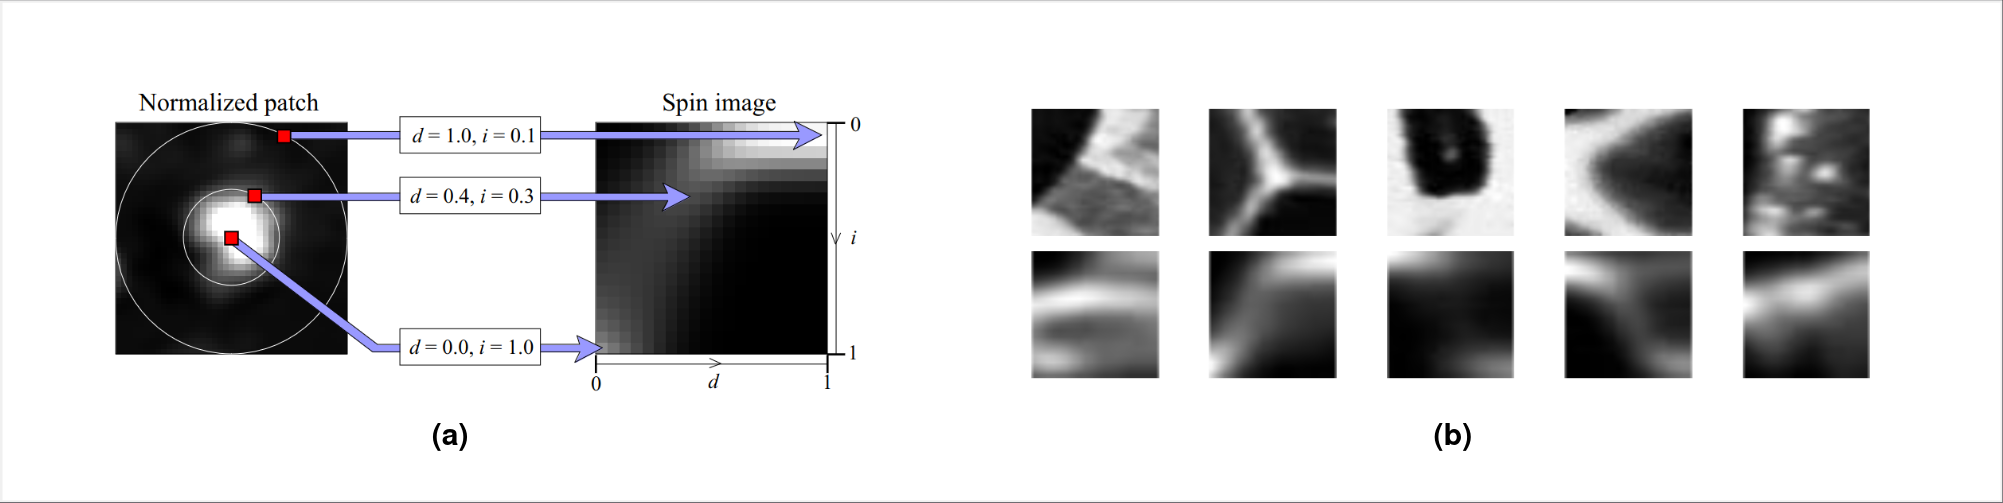
\includegraphics[width=\textwidth]{spin_image.png}
    \caption{\text{Spin} изображение: \textit{(a)} визуализация на съотнасяне между пиксел и кофа от хистограма; \textit{(b)} примерни \textit{spin} изображения; изображенията са собственост на \cite{spinimages}}
    \label{fig:spinim}
\end{figure}

\bigbreak

Подходът за изграждане на \textit{spin} изображения, избран в статия \cite{spinimages} не е перфектен. За всеки пиксел от нормализирания регион се обхожда всяка кофа от хистограмата. Следователно алгоритъмът е с висока времева сложност. При разпределение на приноса на пиксел с координати $\begin{bmatrix} d_0 \\ i_0 \end{bmatrix}$ към кофите от хистограмата се наблюдава, че колкото по-отдалечена е една кофа от $\begin{bmatrix} d_0 \\ i_0 \end{bmatrix}$, толкова по-малко принос получава тя. Съответно в някакъв момент той става неглижируем. Нашата разработка се преборва с този проблем, като прилага обхождане по ширина на матрицата на \textit{spin} изображението, започвайки от клетката с координати най-близки по Евклидово разстояние до $\begin{bmatrix} d_0 \\ i_0 \end{bmatrix}$. При обхождането за терминален връх се счита клетка $\begin{bmatrix} d \\ i \end{bmatrix}$, всички съседи, на която са обходени, или клетка $\begin{bmatrix} d \\ i \end{bmatrix}$, с принос $contrib_{d_0,i_0}(d, i) \leq \varepsilon, \varepsilon \in \mathbb{R}$.

\bigbreak

Друг проблем при предложения от \cite{spinimages} подход за изграждане на \textit{spin} изображения е свързан с наличието на дисбаланс в $d$ оста на изображения. Нека разглеждаме окръжности $O_0$ и $O_1$, съответно с радиуси $r_0$ и $r_1$, такива че $r_0 > r_1$. Очевидно периметъра на $O_0$ е по-голям от този на $O_1$. Това се наблюдава и в алгоритъма за изграждане на \cite{spinimages} изображения. Както споменахме, един нормализиран регион може да се разглежда като множество от концентрични окръжности. Тези по-близо до центъра разполагат с по-малък периметър, съответно по-малко пиксели. Наличието на по-малко пиксели близо до центъра означава, че винаги клетките от \textit{spin} изображението с по-малки $d$ координати ще имат по-малки стойности. Начин да се контрира този проблем е, като се модифицира $contrib_{d_0,i_0}$ функцията. Предлагаме вариант, където $contrib'_{d_0,i_0}(d, i) = \exp(-(d-d_0)^2(2\pi(d_0+\varepsilon))/(2\alpha) - (i-i_0)^2/(2\beta))$. Идеята е, че броят клетки на дистанция $d_0$ от центъра на нормализирания регион расте със скоростта на увеличение на периметъра.

\bigbreak

Разполагайки с множество от \textit{spin} изображения (дескриптори) $H, |H|=K, H \in \mathbb{R}^n, n, K \in \mathbb{N},$ за едно изображение $Im$, следващата стъпка включва изграждането на сигнатура за $Im$. Сигнатура дефинираме като крайно множество от претеглени едномерни хистограми $S = \{<V_k, w_k> | V_k \in \mathbb{R}^n, k,n \in \mathbb{N} $ и $\sum_{j=1}^{|S|} w_j = 1 \}$. Една сигнатура може да има произволен брой елементи.

\bigbreak

Начинът за намиране на сигнатура, използван в \cite{spinimages} започва с агломеративно клъстетиране на \textit{spin} изображенията. Избрано е агломеративно клъстериране защото е трудно предварително да бъде определен броя на клъстерите. Нека намерените клъстери са $J$ на брой и обозначим клъстер с $Cluster_j, 1 \leq j \leq J, j \in \mathbb{N}$. Нека броят на \textit{spin} изображенията причислени към $Cluster_j$ обозначим с $|Cluster_j|$. Тогава причисляваме тегло $w_j$ към $Cluster_j$, такова че $w_j = \frac{|Cluster_j|}{|H|}$, където $|H|$ е броят на всички \textit{spin} изображения. След това за всеки клъстер $Cluster_j$ откриваме центъра или т.нар. медоид чрез формулата $Medoid_j = \frac{\sum_{H \in Cluster_j} H}{|Cluster_j|}$. Намерената сигнатура е $\{<Medoid_1, w_1>, <Medoid_2, w_2>, \cdots, <Medoid_J, w_J>\}$.

\bigbreak

Слабост на избрания подход е, че класическото агломеративно клъстериране не се справя с откриване на клъстери с форма различна от хиперсферична. За да се преборим с този проблем в нашето решение предлагаме използване на \textit{HDBSCAN} (виж \cite{hdbscan}).

\bigbreak

Задачата за откриване на подобни изображения включва предварително изграждане на база от сигнатурите на всички изображения, сред които търсим подобни на входно такова. Нека наречем изображенията в базата предварителни. За всяко предварително изображение се запаметява изображението, заедно с неговата сигнатура. Детайли относно персистентност на решението могат да бъдат открити в следващите секции. Имплементацията предоставя възможност за търсене на $n, n \in \mathbb{N}$, най-сходни изображения на дадено входно на база неговата сигнатура. Следователно трябва да намерим начин за сравнение между две сигнатури.

\bigbreak

Решението предложено в \cite{spinimages} разглежда адаптация на \textit{Earth Mover's Distance (EMD)} като метрика за сравнение между две сигнатури. Нека имаме две сигнатури, съотевтно $\{(\mathbf{m_i}, u_i)\}$ и $\{(\mathbf{n_j}, v_j)\}$. \textit{EMD} стойността между двете се намира използвайки $\frac{\sum_i \sum_j f_{ij} d(\mathbf{m_i}, \mathbf{n_j})}{\sum_i \sum_j f_{ij}}$, където $f_{ij}$ са потокови стойности (\textit{flow values}), намерени чрез решаване на проблем за линейно програмиране, и $d(\mathbf{m_i}, \mathbf{n_j})$ е земната дистанция (\textit{ground distance}) между медоидите $\mathbf{m_i}$ и $\mathbf{n_j}$. Статията не изпада в допълнителни детайли като реферира към \cite{metricfordistributionsforims} и \cite{imretrievalwithoutsegmentation} за насоки относно имплементация на \textit{EMD}.

\bigbreak

Методът \textit{EMD} е още познат като метрика на Васерщайн. В практиката тя най-често бива използвана за намиране на близост между две хистограми. Нека $\mathbf{m}$ и $\mathbf{n}$ са две едномерни хистограми с еднаква размерност. Най-лесният начин да разберем \textit{EMD} е като си въобразим, че стойностите на случайните променливи от $\mathbf{n}$ олицетворяват купчини с пръст, а тези на $\mathbf{m}$ олицетворяват дупки. Пръстта е равна по обем на дупките. Нека разгледаме случайна променлива $i$ от $\mathbf{n}$ и случайна променлива $j$ от $\mathbf{m}$. Цената за пренос на единица пръст от $i$ към $j$ е равна на $|i-j|$. Следователно цената за пренос на пръст между еднакви случайни променливи е $0$. Задачата е да се запълнят дупките с пръст за минимална цена. \textit{EMD} е равно на минималната цена. Налични са множество библиотеки предоставящи решения на \textit{EMD} в този конкретен сценарий. Илюстрация на \textit{EMD} може да бъде открита на фигура \ref{fig:emdandreduction}.

\bigbreak

Намиране на близост между сигнатури, директно прилагайки \textit{EMD} е възможно, чрез дефинирането на проблем за линейно програмиране. \cite{metricfordistributionsforims} и \cite{imretrievalwithoutsegmentation} предоставят идеи, как може да бъде постигнато това чрез редукция до задача за минимална цена на мрежови поток (\textit{minimum cost network flow problem}) (или т.нар. оптимален поток). Задача от такъв вид може да бъде решена чрез линейно програмиране. Стандартен метод е използването на симплекс метода, но както ще покажем по-късно той е неоптимален. За целта ще дефинираме негова специализация над задачи за намиране на оптимален мрежови поток, наречена мрежови симплекс метод (\textit{network simplex method}).

\bigbreak

Ще започнем с дефиницията на това, какво е \textbf{потокова мрежа} (\textit{flow network}). Потокова мрежа наричаме ориентиран граф, където всеки връх притежава \textbf{ресурс}, който се пренася до съседните върхове чрез ребра. Всяко ребро има \textbf{капацитет} над максималния брой единици ресурс, които може да пренесе, както и цена за пренос на единица ресурс. Пренесения ресурс от ребро още наричаме поток на реброто. При някои задачи се допуска този капацитет да бъде безкрайност. Често ребрата биват наричани арки. Ресурсът притежаван от даден връх може да бъде положителен или отрицателен. Може да си мислим, че положителна стойност на ресурс означава излишък на ресурс, а отрицателна - недостиг. Граф където сумата от ресурсите на всички върхове е $0$ се нарича \textbf{балансиран}. 

\bigbreak

Нека имаме граф $G(V, E)$, ресурсът на връх $v \in V$ обозначаваме чрез $supply(v)$ и цената за пренос на единица ресурс през ребро $(u, v) \in E$ чрез $d_{uv}$. Потокът пренесен върху ребро $uv: (u, v) \in E$, обозначаваме чрез $x_{uv}$. Решение на задача върху потокови мрежи наричаме разпределение на потока, такова че за всеки връх $v \in V$ е изпълнено $\sum_{w: (v, w) \in E} x_{vw} - \sum_{u: (u, v) \in E} x_{uv} = supply(v) \iff \sum_{w: (v, w) \in E} x_{vw} - \sum_{u: (u, v) \in E} x_{uv} - supply(v) = 0$. Задачите се различават по параметрите, които оптимизират. Например задачата за намиране на минимален мрежови поток търси разпределение на пренесения поток, такова че $\sum_{(u, v) \in E} d_{uv} x_{uv}$ е минимално. Задачите над потокови мрежи намират редица приложения - логистични задачи, пренос на енергия в затворена система, пренос на течности по тръби и други.

\bigbreak

Нека разгледаме как можем да интерпретираме сравнение между две хистограми чрез \textit{EMD} като задача за намиране на минимална цена в потокова мрежа. Нека $\mathbf{m}$ и $\mathbf{n}$ са нормирани дискретни едномерни хистограми със случайни величини $\{1, 2, \cdots, n\}, n \in \mathbb{N}$. Стойността на случайна величина $j$ от $\mathbf{m}$ означаваме чрез $\mathbf{m}(j)$. Аналогично за $\mathbf{n}$. Нека всяка случайна величина $j$ от $\mathbf{m}$ представим като връх $w_j \in V$ в потокова мрежа $G(V, E)$ с ресурс $supply(w_j) = \mathbf{m}(j)$. Случайна величина $i$ от $\mathbf{n}$ представяме като връх $u_i \in V$ в потокова мрежа $G(V, E)$ с ресурс $supply(u_i) = -\mathbf{n}(i)$. Понеже хистограмите са нормирани, получената потокова мрежа е балансирана. Нека цената за пренос на почва от случайна величина $j$ в $\mathbf{m}$ до случайна величина $i$ в $\mathbf{n}$ представим като ориентирано ребро $(w_j, u_i) \in E$, такова че цената му е $|i - j|$. По този начин сведохме входните данни на \textit{EMD} до потокова мрежа $G$. Може да се докаже, че решението на \textit{EMD} е еквивалентно на решение за минимимална цена в потокова мрежа $G$. Интересно наблюдение е, че $G$ е бипартитен граф, с ребра излизащи от множество $W, W \subset V$ и влизащи в множество $U, U \subset V$. Върховете от $W$ са асоциирани само със случайни величини от $\mathbf{m}$, а тези от $U$ - $\mathbf{n}$. Следователно $W$ представя хистограма $\mathbf{m}$, а $U$ - $\mathbf{n}$. Илюстрация на редукцията може да бъде намерена на фигура \ref{fig:emdandreduction}. Доказахме, че \textit{EMD} е частен случай на задача за намиране на минимална цена в потокова мрежа.

\begin{figure}[ht]
    \centering
    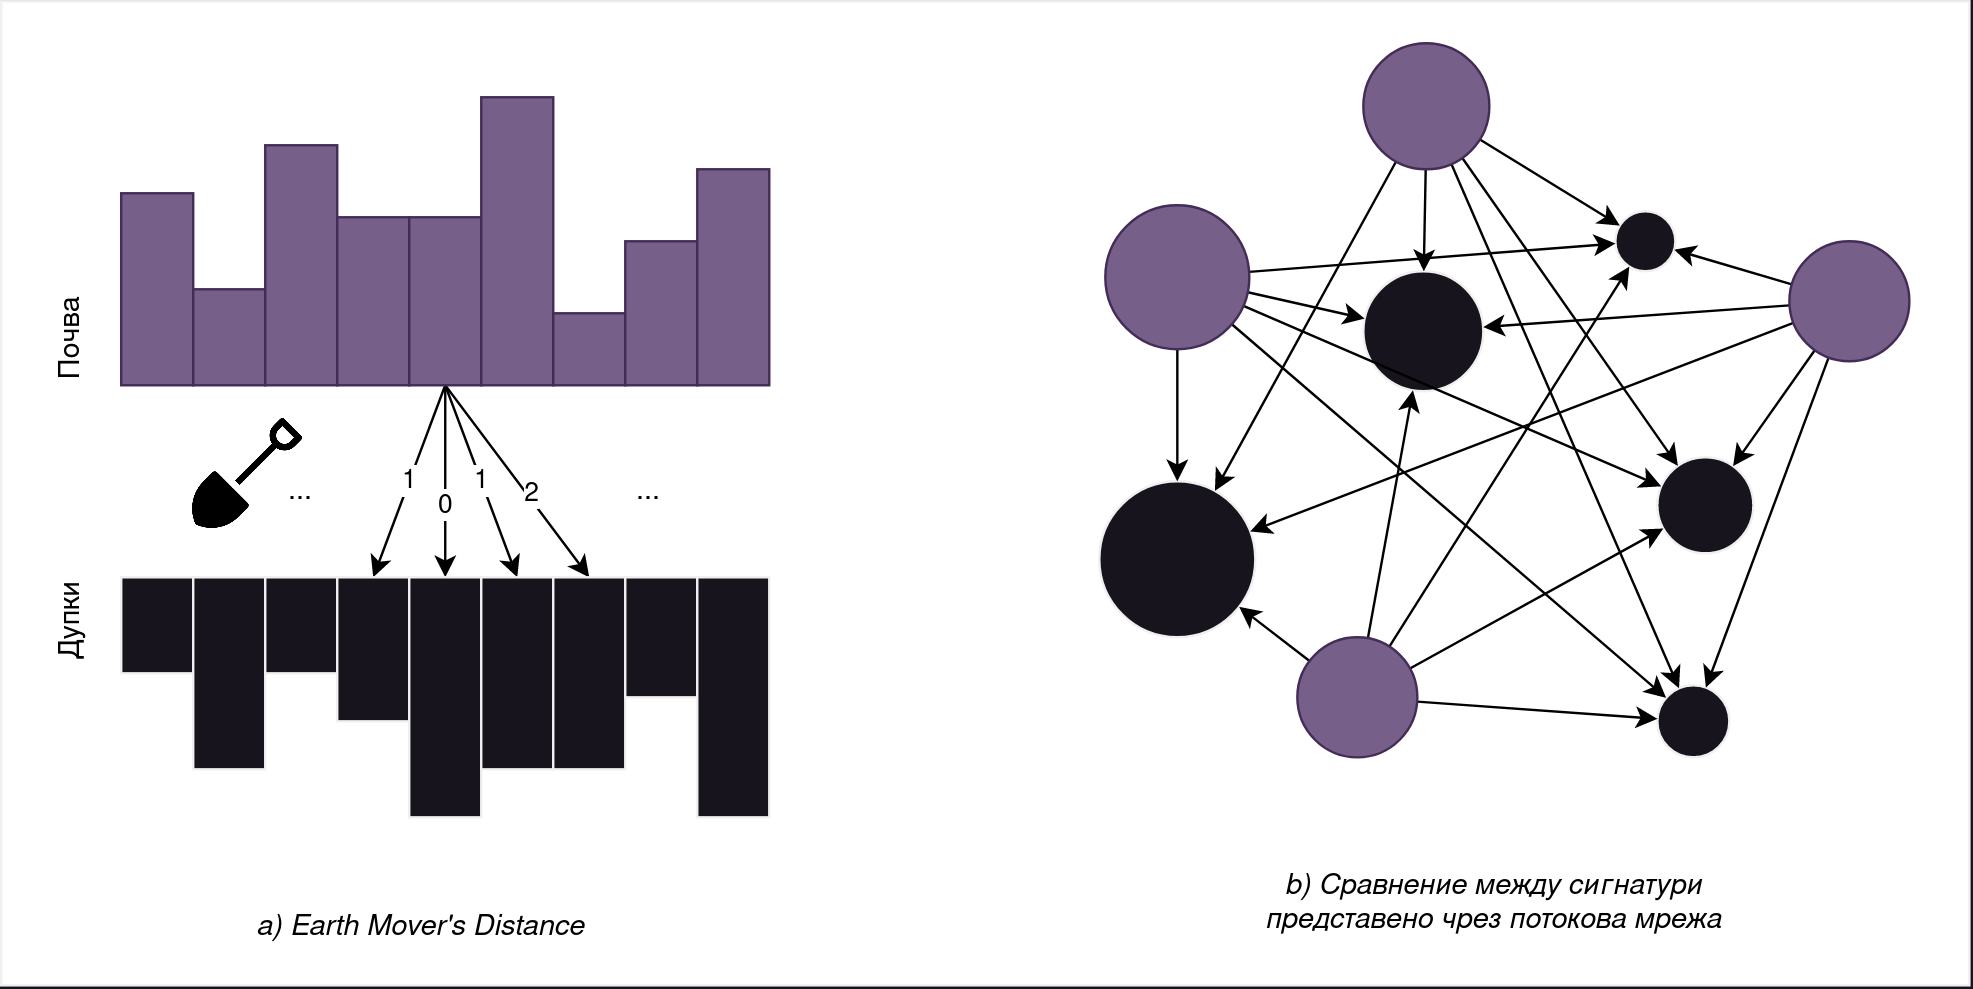
\includegraphics[width=\textwidth]{emd_and_reduction.png}
    \caption{\textit{(a)} \textit{Earth Mover's Distance (EMD)} приложен за сравнение на хистограми. Лилавите стълбчета са почвата, която трябва да бъде пренесена в черните дупки. Интерпретацията за физическа отдалеченост се имплементира посредством теглата на ребрата; \textit{(b)} Редукция на \textit{EMD} до задача за минимална цена на потокова мрежа. Лилавите върхове са почвата, която трябва да бъде пренесена в черните дупки. Радиусът на всеки връх илюстрира размера на неговия ресурс. Дължината на всяко ребро на фигурата илюстрира физическата дистанция между върховете.}
    \label{fig:emdandreduction}
\end{figure}

\bigbreak

Задачата за сравнение на две сигнатури $\mathbf{\alpha} = \{(\mathbf{med}_j, \mathbf{weight}_j)\}$ и $\mathbf{\beta} = \{(\mathbf{med}_i, \mathbf{weight}_i)\}$ не може да се редуцира до \textit{EMD} за сравнение на вектори с еднаква размерност, защото е възможно сигнатурите да са с различни кардиналности. Въпреки това е възможно да я редуцираме до задача за намиране на минимална цена в потокова мрежа използвайки похват подобен на този разгледан преди малко. Нека дефинираме потокова мрежа $G(V, E)$. За всяка двойка $(\mathbf{med}_j, \mathbf{weight}_j) \in \mathbf{\alpha}$ дефинираме връх $w_j \in V$ с ресурс $supply(w_j) = \mathbf{weight}_j$. За всяка двойка $(\mathbf{med}_i, \mathbf{weight}_i) \in \mathbf{beta}$ дефинираме връх $u_i \in V$ с ресурс $supply(u_i) = -\mathbf{weight}_i$. Понеже сумата от всички тегла асоциирани с медоиди в дадена сигнатура е нормирана (сумират се до $1$), получаваме, че $G$ е балансирана. Нека изберем случайно $(\mathbf{med}_j, \mathbf{weight}_j) \in \mathbf{\alpha}$ и $(\mathbf{med}_i, \mathbf{weight}_i) \in \mathbf{beta}$. Знаем, че векторите $\mathbf{med}_j$ и $\mathbf{med}_i$ са с една размерност. Следователно цената за пренос на ресурс от връх $w_j$ до връх $u_i$ представяме като ребро $(w_j, u_i) \in E$, такова че неговата цена е $\lVert u_i - w_j \rVert$. По този начин сведохме входните данни на задачата за намиране на близост между две сигнатури до потокова мрежа $G$. Може да се докаже, че намирането на минимална цена в на потокова мрежа $G$ дава решението на \textit{EMD} за сравнение на вектори с различна размерност. Както преди, забелязваме, че $G$ е бипартитен, като можем да го разделим на две множества, съответно $W$ и $U$. Върховете от $W$ са асоциирани с елементи на $\mathbf{\alpha}$, а тези от $U$ - $\mathbf{\beta}$.  Илюстрация на редукцията може да бъде намерена на фигура \ref{fig:emdandreduction}.


% #############################################################################################################
\subsubsection{Инвариантна към мащаби трансформация на атрибути в комбинация с $k$ най-близки съседи}

Инвариантна към мащаби трансформация на свойства (\textit{Scale Invariant Feature Transform (SIFT)}) е един от най-успешните подходи за откриване на точки на интерес. Те са инвариантни към скалиране, ротация, отместване и частично инвариантни към промяна на илюминация и локална дисторция.  Откритите точки на интерес се явяват като апроксимация на тези, открити от главната визуална кора на приматите по това, че споделят подобно кодиране на форми и цвят (виж \cite{primatevisualcortex}). SIFT е разделен на няколко стъпки - откриване на потенциални точки на интерес, тяхната филтрация и присвояване на съответно векторно представяне.

\bigbreak

За да се открият потенциалните точки на интерес в изображение $I$ се започва с изграждането на \textbf{пространство на мащабите}. Намират се $n$ на брой октави на $I$, където над всяка октава, $k+1$ пъти последователно е приложен Гаусов филтър. Приложеният филтър на стъпка $s$ е със стандартно отклонение $\sigma_s, 0 <= s < k+1, s \in \mathbb{N}$, където $\sigma_{s+1} = 1.6 \sigma_s$. За всяка октава $i$ намираме разликата между всеки две последователно Гаусови филтрирания $j$ и $j+1$ (т.нар. разлика между Гаусови филтрирания (\textit{Difference of Gaussians (DoG)})), където $i < n, j < k, i, j \in \mathbb{N}$. Съответно пространството на мащабите се състои от $nk$ на брой изображения (виж фиг.). Нека интензитетът на точка $(x, y)$ на изображението от $j$-тото ниво на $i$-тата октава означим като $I_{ij}(x,y)$.

\bigbreak

Получените изображения апроксимират прилагането на Лапласов оператор, при който изпъкват очертанията на фигурите. Друга аналогия, ако разглеждаме $I$ като сигнал, е тази с \textit{band-pass filter}, защото прилагането на Гаусов филтър премахва високите честоти, а $DoG$ премахва честотите от по-замъгленото изображение (т.е. ниските). С други думи всяко ниво от пространството на мащабите представя конкретен честотен интервал на входното изображение $I$. За всеки такъв интервал \textit{SIFT} открива екстремални точки, които са потенциални точки на интерес. Една точка $(x, y)$ от $I_{ij}$ наричаме екстремална, ако за интензитетът ѝ $I_{ij}(x, y)$ е изпълнено $I_{ij}(x, y) >= I_{(i+r)(j+p)}(x+n, y+m) \forall r,p,n,m \in \{-1, 0, 1\}$. Тогава ако релацията за съседство дефинирана над изображението е $8$-съседство, се правят $9+8+9=26$ сравнения (виж фиг.).

\bigbreak

Някои от откритите до тук екстремални точки е възможно да са нестабилни спрямо трансформации, съответно е желателно те да бъдат премахнати. За подобрена точност, при процеса на филтрация, сигнала на изображението се конвертира от дигитален в аналогов. Точната локация на всеки екстремум $p=(x, y)$ за изображение $I_{ij}$ се апроксимира чрез \textbf{развитие на Тейлър} с център на координатната система $(x, y, \sigma_j)$: \\

$D(\varphi) = D + \frac{\partial D^T}{\partial \varphi}\varphi + \frac{\varphi^T}{2}\frac{\partial^2 D}{\partial \varphi^2}\varphi$ \\

, където $\sigma_j$ е стандартното отклонение за $I_{ij}$ и $\varphi=(x_{offset},y_{offset},\sigma_{offset})^T$ е отместване спрямо центъра на координатната система. Отместването към аналоговия екстремум $\hat{\varphi}$ намираме чрез откриване на корените на $D'$. Ако $max(\lvert\hat{\varphi}\rvert) > 0.5$, то истинският екстремум е по-близо до друга точка на интерес. Следователно изчисляваме наново $D$ с център на координатната система $(x, y, \sigma_j) + \hat{\varphi}$ и повтаряме итеративно процеса. В противен случай приемаме, че отместването на екстремума е $\hat{\varphi}$.

\bigbreak

Ако един екстремум не е достатъчно изпъкнал, т.е. $D''(\hat{\varphi}) < 0.03$, то се предполага, че той е нестабилен. Следва елиминация на точки намиращи се върху ръбове, където се използват характеристичните стойности на Хесиановата матрица на $D$. Новата локация на точката на интерес след процеса на филтрация е $(x, y, \sigma_j) + \hat{\varphi}$.

\bigbreak

Предните стъпки подсигуряват инвариантност към отместване и скалиране. Чрез тази стъпка се постига инвариантност към ротация на изображението. За дадена точка на интерес $(x, y)$ от октава $i$ със стандартно отклонение $\sigma$ наричаме съответното Гаусово филтриране $I_{\sigma}$. В околност около $(x, y)$ намираме размера и ориентацията на всеки градиент: \\

$m(x', y') = \sqrt{(I_{\sigma}(x'+1,y') - I_{\sigma}(x'-1,y'))^2 + (I_{\sigma}(x', y'+1) - I_{\sigma}(x', y'-1))^2}$ \\
$\theta(x', y') = \arctan(I_{\sigma}(x',y'+1) - I_{\sigma}(x',y'-1), I_{\sigma}(x'+1,y') - I_{\sigma}(x'-1, y'))$ \\

Създава се хистограма с 36 кофи, всяка съответстваща на интервал от $10\degree$. Всяка точка $(x', y')$ от околността $(x, y)$ се причислява към конкретна кофа според ориентацията си, като добавената стойността се претегля според магнитута и стандартното отклонение. Намира се теглото на най-тежката кофа, като оцеляват само кофите с тегло поне $0.8$ от теглото на най-тежката кофа. За всяка оцеляла кофа се създава ключова точка с тази ориентация.

\bigbreak

За изграждането на финалния дескриптор на точка на интерес се взима регион с размер $16 \times 16$ около нея. Той се разбива на 16 подрегиона, всеки с размер $4 \times 4$. За всеки регион се създава хистограма с 8 кофи. Съответно всеки дескриптор на точка на интерес има размерност $16 \times 8 = 128$. Подобно на предната стъпка, за всяка точка от този регион се намира ориентация и магнитут. За инвариантност на ротацията и отместването се използват координатната система на точката на интерес, чиито дескриптор се пресмята. За добавена инвариантност към илюминация се извършва нормализация и подрязване на финалния дескриптор.

% #############################################################################################################
\subsubsection{Бързо търсене на подобни изображения чрез лексикално дърво}

Този подход се базира над \cite{vocabularytree}.

\subsection{Съществуващи решения (практически реализации)}

\subsection{Избор на критерии за сравнение и сравнителен анализ на решения}

\subsection{Изводи}

% =============================================================================================================
\section{Използвани технологии, платформи и/или методологии}

% =============================================================================================================
\section{Анализ}

% =============================================================================================================
\section{Проектиране}

% =============================================================================================================
\section{Реализация, тестване/експерименти и внедряване}

% =============================================================================================================
\section{Заключение}

% =============================================================================================================
\printbibliography[title={Използвана литература}]

\end{document}
